\documentclass[11pt,a4paper,openright,twoside]{article}
\usepackage[english]{babel}
\usepackage{newlfont}
\usepackage{color}
\textwidth=450pt\oddsidemargin=0pt
\usepackage{graphicx}
\usepackage{float}
\usepackage{textcomp}
\usepackage{caption}
\usepackage{wrapfig}
\usepackage{subfig}
\usepackage{sidecap}
\usepackage[rlft]{floatflt}
\usepackage{amsmath}
\usepackage{amssymb}
\usepackage{bm}
\usepackage{fancyhdr}
\usepackage{multirow}
\usepackage[utf8x]{inputenc}
\usepackage{fullpage}
\usepackage[Lenny]{fncychap}
\usepackage[T1]{fontenc}
\usepackage[normalem]{ulem}
\usepackage{booktabs}
\usepackage{enumerate}
\usepackage{tikz}
\usetikzlibrary{positioning}

\tikzset{c-rectangle2/.style={rectangle, rounded corners, minimum width=2cm, minimum height=1cm, text centered, text width=4cm, draw=black, fill=white},
arrow/.style={thick,->,>=stealth}}


%\usepackage[usenames,dvipsnames]{xcolor}
%\usepackage{listings}
%\usepackage{xcolor}

%\definecolor{light-gray}{gray}{0.95}
%\lstset{language=R,
%    basicstyle=\small\ttfamily,
%    stringstyle=\itshape\color{RedViolet},
%    showstringspaces=false,
%    otherkeywords={0,1,2,3,4,5,6,7,8,9},
%    morekeywords={TRUE,FALSE, ggplot, data.frame, theme, ylab, xlab},
%    deletekeywords={data, frame, beta, c, par, colours, contour, scale,
%                    panel, grid, hat},
%    keywordstyle=\color{RoyalBlue},
%    commentstyle=\itshape\color{PineGreen},
%    backgroundcolor=\color{light-gray}
%}



\title{CTRP - A Toy Example}
\author{}
\date{}





\begin{document}

\maketitle

\section{Data}
Considering $f=5$ predictors and $B=10$ permutations, we simulate a $B\times f$ matrix of global test statistics:

\begin{table}[h!]
\centering
\begin{tabular}{ccccc}
\multicolumn{5}{c}{$\mathbf{G}$}\\
$(1)$ & $(2)$ & $(3)$ & $(4)$ & $(5)$\\
\cline{1-5}
28.42 & 16.68 & 9.36 & 6.12 & 9.40\\
0.10 & 0.06 & 1.37 & 0.08 & 0.56\\
0.69 & 3.07 & 4.33 & 0.83 & 0.36\\
1.07 & 30.31 & 1.11 & 8.55 & 0.26\\
0.22 & 7.45 & 2.87 & 0.48 & 1.02\\
1.83 & 0.04 & 2.85 & 0.04 & 0.02\\
17.68 & 1.82 & 6.00 & 1.52 & 1.06\\
1.77 & 26.12 & 0.29 & 0.26 & 4.07\\
2.71 & 0.37 & 8.47 & 5.83 & 4.42\\
1.14 & 0.03 & 24.06 & 8.84 & 2.41\\
\end{tabular}
\end{table}

Assume that we want to test $S=\{5\}$ with significance level $\alpha=0.20$.




\vspace{10mm}
\section{Shortcut}
\begin{table}[h!]
\centering
\resizebox{\textwidth}{!}{
\begin{tabular}{c|ccccccccccc}
v &   &  &  &  &  &  &  &  &  &  &  \\
4 &  &  &  &  &  & $\mathbf{F=\{1,2,3,4,5\}}$ &  &  &  &  &  \\
3 &  &  & $\{1,2,3,5\}$ &  & $\{1,2,4,5\}$ &  & $\{1,3,4,5\}$ &  & $\mathbf{\{2,3,4,5\}}$ &  &  \\
2 & $\{1,2,5\}$  &  & $\{1,3,5\}$ &  & $\{1,4,5\}$ &  & $\{2,3,5\}$ &  & $\{2,4,5\}$ &  & $\mathbf{\{3,4,5\}}$ \\
1 &  &  & $\{1,5\}$ &  & $\{2,5\}$ &  & $\{3,5\}$ &  & $\mathbf{\{4,5\}}$ &  &  \\
0 &  &  &  &  &  & $\mathbf{S=\{5\}}$ &  &  &  &  &  
\end{tabular}
}
\caption{Supersets of $S=\{5\}$, having sizes $|V|=1+v$ with $v=0,\ldots,4$. The sets in bold are used to define the lower critical value $L_v$.}
\end{table}

We define
\begin{itemize}
\item $\mathbf{D}$, matrix of the centered test statistics in $F\setminus S$, where the indices appear in the order $(4,3,2,1)$ (since $g_4\leq g_3\leq g_2\leq g_1$);
\item $\mathbf{R}$, matrix obtained from $\mathbf{D}$ by sorting the elements within each row in decreasing order.
\end{itemize}

\newpage
\begin{table}[h!]
\centering
%\resizebox{\textwidth}{!}{
\begin{tabular}{ccccccccccc}
$\mathbf{d}_S$ & & \multicolumn{4}{c}{$\mathbf{D}$} & & \multicolumn{4}{c}{$\mathbf{R}$}\\
$(5)$ &  & $(4)$ & $(3)$ & $(2)$ & $(1)$ &  &  &  &  &  \\
\cline{1-1} \cline{3-6} \cline{8-11}
0.00 &  & 0.00 & 0.00 & 0.00 & 0.00 &  & 0.00 (1)& 0.00 (2)& 0.00 (3)& 0.00 (4)\\
-8.84 &  & -6.03 & -7.99 & -16.62 & -28.32 &  & -6.03 (4)& -7.99 (3)& -16.62 (2)& -28.32 (1)\\
-9.04 &  & -5.29 & -5.02 & -13.61 & -27.72 &  & -5.02 (3)& -5.29 (4)& -13.61 (2)& -27.72 (1)\\
-9.14 &  & 2.43 & -8.25 & 13.63 & -27.34 &  & 13.63 (2)& 2.43 (4)& -8.25 (3)& -27.34 (1)\\
-8.38 &  & -5.63 & -6.49 & -9.23 & -28.19 &  & -5.63 (4)& -6.49 (3)& -9.23 (2)& -28.19 (1)\\
-9.38 &  & -6.08 & -6.51 & -16.64 & -26.59 &  & -6.08 (4)& -6.51 (3)& -16.64 (2)& -26.59 (1)\\
-8.34 &  & -4.59 & -3.36 & -14.86 & -10.74 &  & -3.36 (3)& -4.59 (4)& -10.74 (1)& -14.86 (2)\\
-5.33 &  & -5.85 & -9.07 & 9.44 & -26.65 &  & 9.44 (2)& -5.85 (4)& -9.07 (3)& -26.65 (1)\\
-4.98 &  & -0.28 & -0.89 & -16.31 & -25.71 &  & -0.28 (4)& -0.89 (3)& -16.31 (2)& -25.71 (1)\\
-6.99 &  & 2.72 & 14.70 & -16.65 & -27.27 &  & 14.70 (3)& 2.72 (4)& -16.65 (2) & -27.27 (1)
\end{tabular}
%}
\end{table}

The lower and upper critical values, $L_v$ and $U_v$, are the 8-th ordered statistics of
\begin{align*}
& \mathbf{d}_{\tilde{V}}=\mathbf{d}_3 + \sum_{i=1}^v \mathbf{D}_i & \mathbf{u}_v=\mathbf{d}_3 + \sum_{i=1}^v \mathbf{R}_i.
\end{align*}

Since the first column of $\mathbf{R}$ having no positive elements has index $w=3$, we start by computing $L_v$ for $v=0,1,2$.

No non-rejection is found, and thus we proceed by examining $v>2$, until we find either a rejection or a negative $U_v$. Here $U_v$ becomes negative for $v=3$, hence the supersets with $v=3,4$ are automatically rejected.

Finally, we determine the indecisive values by looking at $U_v$. Here they are $v=1,2$.

\begin{figure}[h!]
\centering
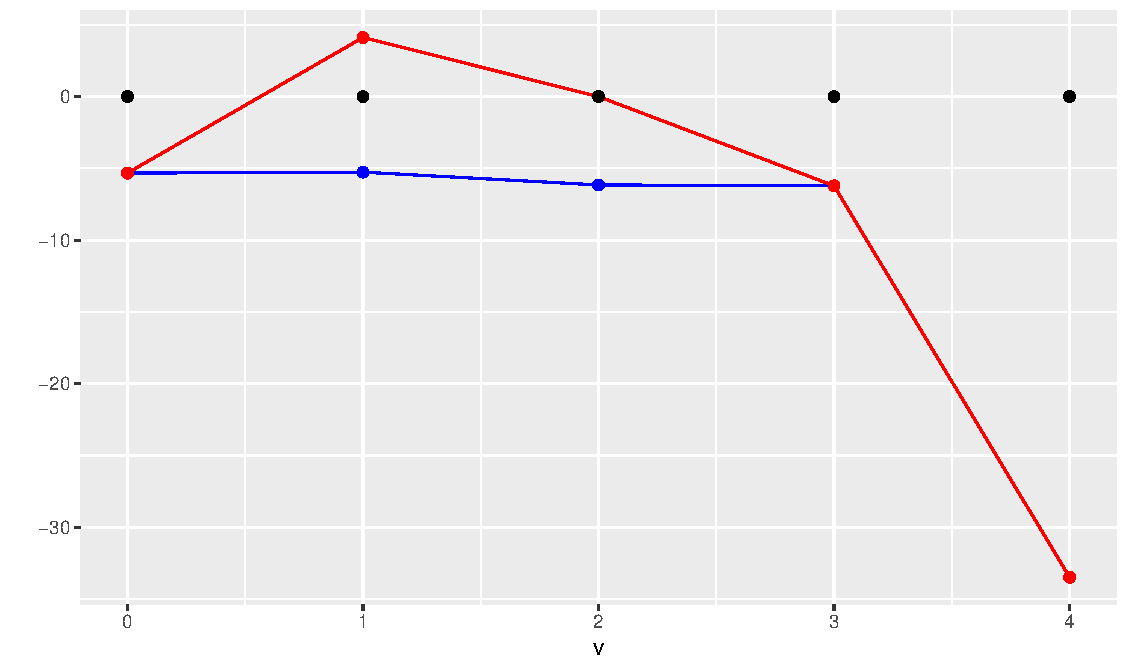
\includegraphics[scale=0.57]{plot1.pdf}
\caption{Upper (red) and lower (blue) critical values and observed values (zero, black) by additional superset size $v$. The bounds for $v=4$ have not been computed in the analysis.}
%\label{fig:bounds}
\end{figure}


\begin{table}[h!]
\centering
\begin{tabular}{cccccc}
\toprule
$v$ & 0 & 1 & 2 & 3 & 4\\
\midrule
$U_v$ & -5.33 & 4.11 & 0.00 & -6.22 & (-33.49)\\
$L_v$ & -5.33 & -5.26 & -6.16 & -6.22 & (-33.49)\\
\midrule
rej & T & ? & ? & T & T\\
\bottomrule
\end{tabular}
\end{table}


\newpage
\section{Branch and Bound}
\subsection{Removal of the highest statistic.}
The last index in $\mathbf{D}$, $e=1$, determines the branching rule. We explore first the subspace $\mathbb{S}_{-1}$, where we examine only $U_v$.
\begin{table}[h!]
\centering
\begin{tabular}{c|ccccccc}
 & \multicolumn{3}{c}{$\mathbb{S}_{-1}$} & & \multicolumn{3}{c}{$\mathbb{S}_{+1}$}\\
\cline{2-4} \cline{6-8}
2 & $\{2,3,5\}$ & $\{2,4,5\}$ & $\{3,4,5\}$ & & $\{1,2,5\}$ & $\{1,3,5\}$ & $\{1,4,5\}$ \\
1 & $\{2,5\}$ & $\{3,5\}$ & $\{4,5\}$ & & & $\{1,5\}$ &  \\
\end{tabular}
\end{table}

Since the outcome is still indecisive for both sizes $v=1,2$, the subspace is partitioned again according to the inclusion of $e=2$ (corresponding to the second highest statistic $g_i$).
\begin{table}[h!]
\centering
\begin{tabular}{c|ccccccc}
 & \multicolumn{3}{c}{$\mathbb{S}_{-1,-2}$} & & \multicolumn{3}{c}{$\mathbb{S}_{-1,+2}$}\\
\cline{2-4} \cline{6-8}
2 &  & $\{3,4,5\}$ &  & & $\{2,3,5\}$ &  & $\{2,4,5\}$ \\
1 & $\{2,5\}$ &  & $\{3,5\}$ &  &  & $\{4,5\}$ &  \\
\end{tabular}
\end{table}

Since $S$ is not rejected in $\mathbb{S}_{-1,+2}$, it is not rejected in the total space after 3 steps.

\vspace{10mm}

\begin{figure}[h!]
\centering
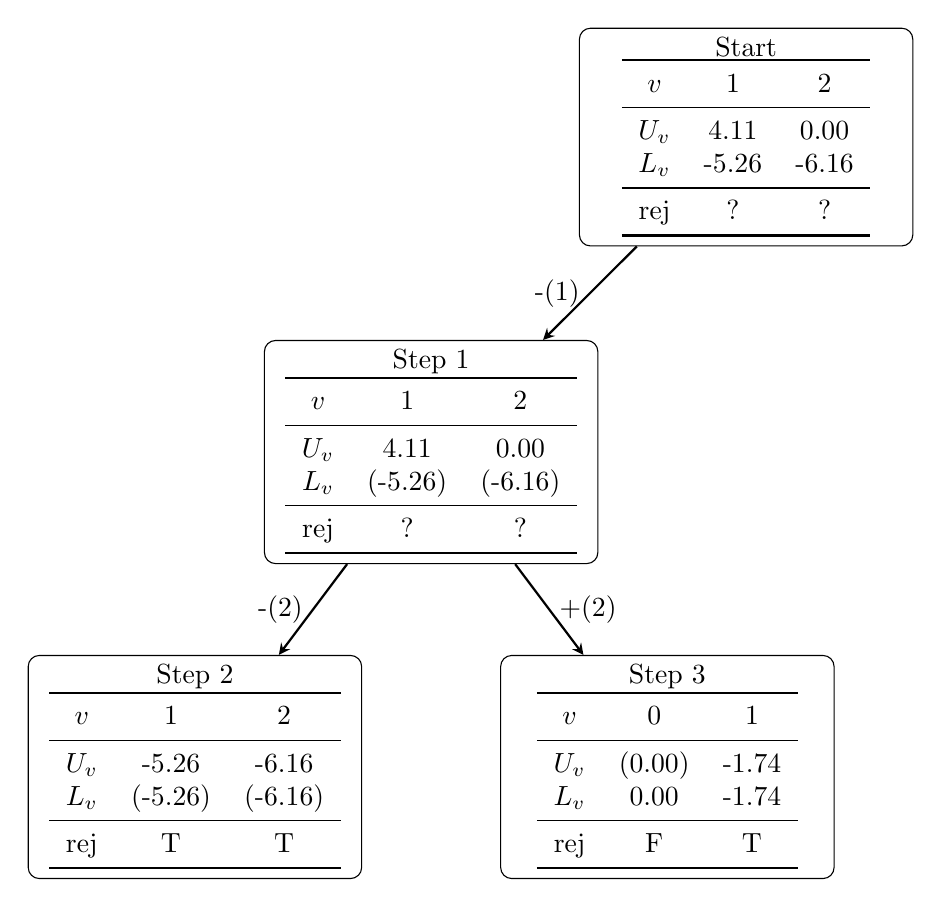
\begin{tikzpicture}[node distance = 4cm]
\node (n0) [c-rectangle2] {Start\\
\begin{tabular}{ccc}
\toprule
$v$ & 1 & 2 \\
\midrule
$U_v$ & 4.11 & 0.00\\
$L_v$ & -5.26 & -6.16\\
\midrule
rej & ? & ?\\
\bottomrule
\end{tabular}
};
\node (n1) [c-rectangle2, below of=n0, xshift=-4cm] {Step 1\\
\begin{tabular}{ccc}
\toprule
$v$ & 1 & 2 \\
\midrule
$U_v$ & 4.11 & 0.00\\
$L_v$ & (-5.26) & (-6.16)\\
\midrule
rej & ? & ?\\
\bottomrule
\end{tabular}
};
\node (n2) [c-rectangle2, below of=n1, xshift=-3cm] {Step 2\\
\begin{tabular}{ccc}
\toprule
$v$ & 1 & 2 \\
\midrule
$U_v$ & -5.26 & -6.16\\
$L_v$ & (-5.26) & (-6.16)\\
\midrule
rej & T & T\\
\bottomrule
\end{tabular}
};
\node (n3) [c-rectangle2, below of=n1, xshift=3cm] {Step 3\\
\begin{tabular}{ccc}
\toprule
$v$ & 0 & 1 \\
\midrule
$U_v$ & (0.00) & -1.74\\
$L_v$ & 0.00 & -1.74\\
\midrule
rej & F & T\\
\bottomrule
\end{tabular}
};
\draw [arrow] (n0) -- node[anchor=east] {-(1)} (n1);
\draw [arrow] (n1) -- node[anchor=east] {-(2)} (n2);
\draw [arrow] (n1) -- node[anchor=west] {+(2)} (n3);
\end{tikzpicture}
%\caption{Illustration of State of the Art}
%\label{fig:Illustration of State of the Art}
\end{figure}






\newpage
\subsection{Keeping of the highest statistic.}
The last index in $\mathbf{D}$, $e=1$, determines the branching rule. We explore first the subspace $\mathbb{S}_{+1}$, where we examine both critical values.

$S$ is not rejected after 3 steps: it is rejected in $\mathbb{S}_{+1}$, but it is not rejected in $\mathbb{S}_{-1,+2}$.

\vspace{10mm}

\begin{figure}[h!]
\centering
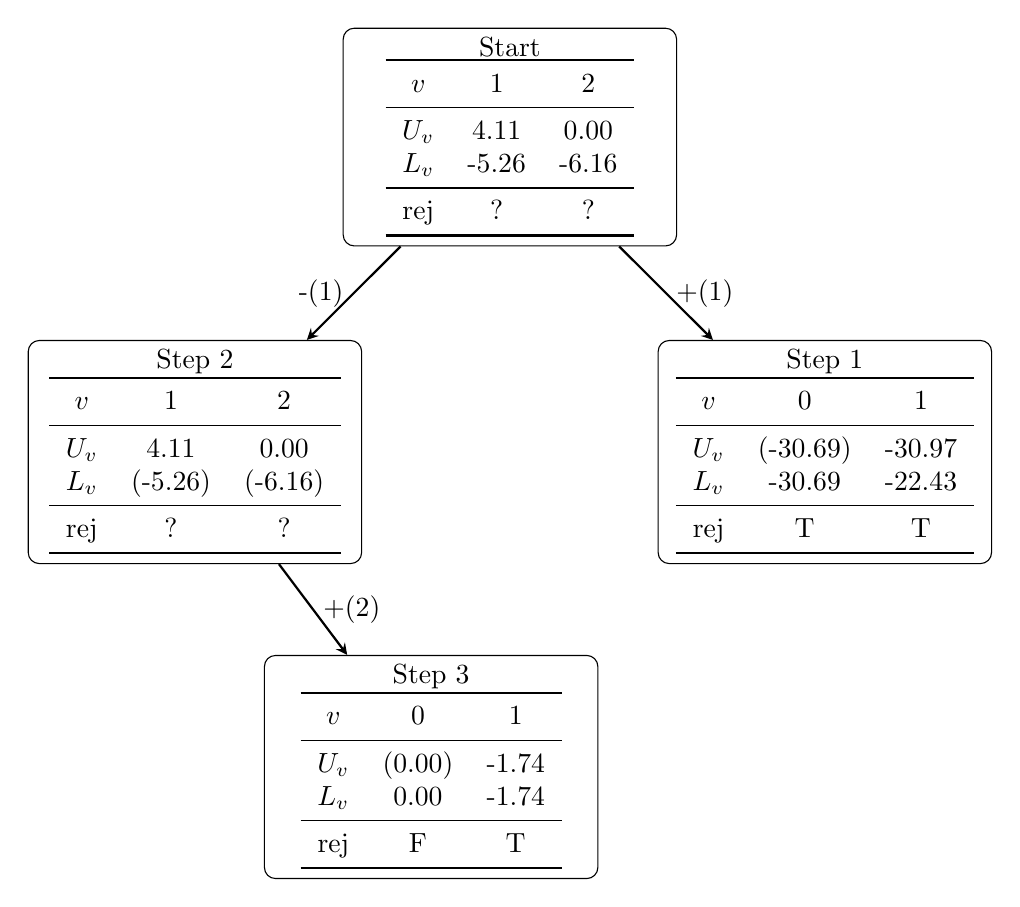
\begin{tikzpicture}[node distance = 4cm]
\node (n0) [c-rectangle2] {Start\\
\begin{tabular}{ccc}
\toprule
$v$ & 1 & 2 \\
\midrule
$U_v$ & 4.11 & 0.00\\
$L_v$ & -5.26 & -6.16\\
\midrule
rej & ? & ?\\
\bottomrule
\end{tabular}
};
\node (n1) [c-rectangle2, below of=n0, xshift=4cm] {Step 1\\
\begin{tabular}{ccc}
\toprule
$v$ & 0 & 1 \\
\midrule
$U_v$ & (-30.69) & -30.97\\
$L_v$ & -30.69 & -22.43\\
\midrule
rej & T & T\\
\bottomrule
\end{tabular}
};
\node (n2) [c-rectangle2, below of=n0, xshift=-4cm] {Step 2\\
\begin{tabular}{ccc}
\toprule
$v$ & 1 & 2 \\
\midrule
$U_v$ & 4.11 & 0.00\\
$L_v$ & (-5.26) & (-6.16)\\
\midrule
rej & ? & ?\\
\bottomrule
\end{tabular}
};
\node (n3) [c-rectangle2, below of=n2, xshift=+3cm] {Step 3\\
\begin{tabular}{ccc}
\toprule
$v$ & 0 & 1 \\
\midrule
$U_v$ & (0.00) & -1.74\\
$L_v$ & 0.00 & -1.74\\
\midrule
rej & F & T\\
\bottomrule
\end{tabular}
};
\draw [arrow] (n0) -- node[anchor=west] {+(1)} (n1);
\draw [arrow] (n0) -- node[anchor=east] {-(1)} (n2);
\draw [arrow] (n2) -- node[anchor=west] {+(2)} (n3);
\end{tikzpicture}
%\caption{Illustration of State of the Art}
%\label{fig:Illustration of State of the Art}
\end{figure}





\newpage
\subsection{Removal of the lowest statistic.}
The first index in $\mathbf{D}$, $e=4$, determines the branching rule. We explore first the subspace $\mathbb{S}_{-4}$, where we examine both critical values.

$S$ is not rejected after 2 steps, where the subspaces $\mathbb{S}_{-4}$ and $\mathbb{S}_{-4,-3}$ are explored.

\vspace{10mm}

\begin{figure}[h!]
\centering
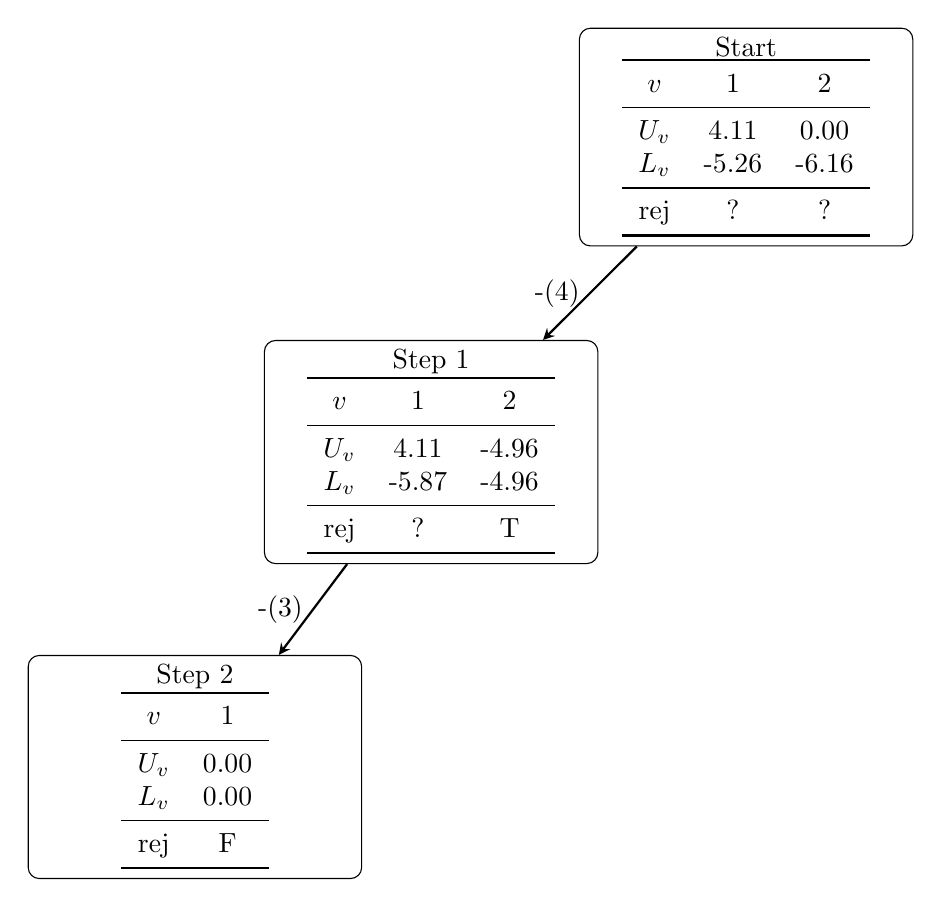
\begin{tikzpicture}[node distance = 4cm]
\node (n0) [c-rectangle2] {Start\\
\begin{tabular}{ccc}
\toprule
$v$ & 1 & 2 \\
\midrule
$U_v$ & 4.11 & 0.00\\
$L_v$ & -5.26 & -6.16\\
\midrule
rej & ? & ?\\
\bottomrule
\end{tabular}
};
\node (n1) [c-rectangle2, below of=n0, xshift=-4cm] {Step 1\\
\begin{tabular}{ccc}
\toprule
$v$ & 1 & 2 \\
\midrule
$U_v$ & 4.11 & -4.96\\
$L_v$ & -5.87 & -4.96\\
\midrule
rej & ? & T\\
\bottomrule
\end{tabular}
};
\node (n2) [c-rectangle2, below of=n1, xshift=-3cm] {Step 2\\
\begin{tabular}{cc}
\toprule
$v$ & 1 \\
\midrule
$U_v$ & 0.00 \\
$L_v$ & 0.00 \\
\midrule
rej & F\\
\bottomrule
\end{tabular}
};
\draw [arrow] (n0) -- node[anchor=east] {-(4)} (n1);
\draw [arrow] (n1) -- node[anchor=east] {-(3)} (n2);
\end{tikzpicture}
%\caption{Illustration of State of the Art}
%\label{fig:Illustration of State of the Art}
\end{figure}






\newpage
\subsection{Keeping of the lowest statistic.}
The first index in $\mathbf{D}$, $e=4$, determines the branching rule. We explore first the subspace $\mathbb{S}_{+4}$, where we examine only $U_v$.

After 2 steps, $S$ is rejected in the subspace $\mathbb{S}_{+4}$. Subsequently, after 2 other steps, it is not rejected in $\mathbb{S}_{-4}$. In conclusion, it is not rejected after 4 steps.

\vspace{10mm}

\begin{figure}[h!]
\centering
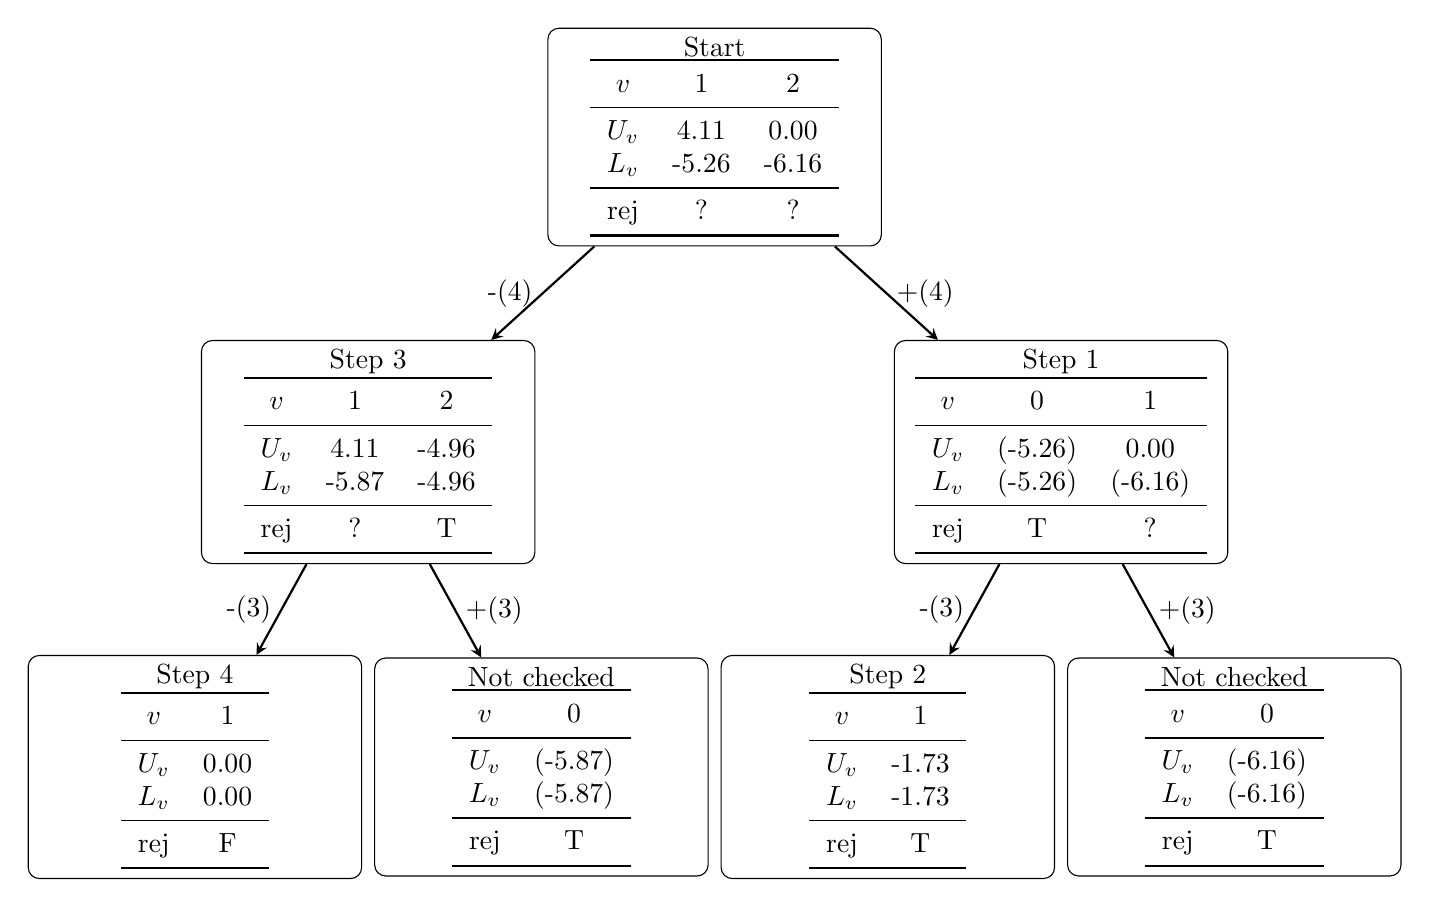
\begin{tikzpicture}[node distance = 4cm]
\node (n0) [c-rectangle2] {Start\\
\begin{tabular}{ccc}
\toprule
$v$ & 1 & 2 \\
\midrule
$U_v$ & 4.11 & 0.00\\
$L_v$ & -5.26 & -6.16\\
\midrule
rej & ? & ?\\
\bottomrule
\end{tabular}
};
\node (n1) [c-rectangle2, below of=n0, xshift=4.4cm] {Step 1\\
\begin{tabular}{ccc}
\toprule
$v$ & 0 & 1 \\
\midrule
$U_v$ & (-5.26) & 0.00\\
$L_v$ & (-5.26) & (-6.16)\\
\midrule
rej & T & ?\\
\bottomrule
\end{tabular}
};
\node (n2) [c-rectangle2, below of=n1, xshift=2.2cm] {Not checked\\
\begin{tabular}{cc}
\toprule
$v$ & 0\\
\midrule
$U_v$ & (-6.16)\\
$L_v$ & (-6.16)\\
\midrule
rej & T \\
\bottomrule
\end{tabular}
};
\node (n3) [c-rectangle2, below of=n1, xshift=-2.2cm] {Step 2\\
\begin{tabular}{cc}
\toprule
$v$ & 1 \\
\midrule
$U_v$ & -1.73\\
$L_v$ & -1.73\\
\midrule
rej & T \\
\bottomrule
\end{tabular}
};
\node (n4) [c-rectangle2, below of=n0, xshift=-4.4cm] {Step 3\\
\begin{tabular}{ccc}
\toprule
$v$ & 1 & 2 \\
\midrule
$U_v$ & 4.11 & -4.96\\
$L_v$ & -5.87 & -4.96\\
\midrule
rej & ? & T\\
\bottomrule
\end{tabular}
};
\node (n5) [c-rectangle2, below of=n4, xshift=2.2cm] {Not checked\\
\begin{tabular}{cc}
\toprule
$v$ & 0 \\
\midrule
$U_v$ & (-5.87) \\
$L_v$ & (-5.87) \\
\midrule
rej & T\\
\bottomrule
\end{tabular}
};
\node (n6) [c-rectangle2, below of=n4, xshift=-2.2cm] {Step 4\\
\begin{tabular}{cc}
\toprule
$v$ & 1 \\
\midrule
$U_v$ & 0.00 \\
$L_v$ & 0.00 \\
\midrule
rej & F\\
\bottomrule
\end{tabular}
};
\draw [arrow] (n0) -- node[anchor=west] {+(4)} (n1);
\draw [arrow] (n1) -- node[anchor=west] {+(3)} (n2);
\draw [arrow] (n1) -- node[anchor=east] {-(3)} (n3);
\draw [arrow] (n0) -- node[anchor=east] {-(4)} (n4);
\draw [arrow] (n4) -- node[anchor=west] {+(3)} (n5);
\draw [arrow] (n4) -- node[anchor=east] {-(3)} (n6);
\end{tikzpicture}
\end{figure}















\end{document}